\documentclass[11pt]{article}

\usepackage[utf8x]{inputenc}
\usepackage[slovene]{babel}

\usepackage{amssymb}
\usepackage{amsmath} 
\usepackage{url}

\usepackage{float}

\usepackage[pdftex]{graphicx} % za slike

\title{\textbf{Robustness of persistence diagrams}}
\author{O\v zbolt Menegatti\\
		Anej Placer\\
		Jurij Slabanja}
\date{}
\begin{document}

\maketitle

\section{Project goal}

The goal of this project was to demonstrate the robustness of persistence diagrams of the Vietoris-Rips complex on a specific example.

\subsection{Vietoris-Rips}
Vietoris-Rips complex is very similar to Cech complex, but here we don't operate with virtual spheres. The distances between pairs of points are used instead. In Vietoris-Rips complex a simplex is part of the complex only if the diameter of the simplex is smaller or equal to $2\delta$ (maximal distance between two points). The difference from the Cech complex is easily observed if we consider vertexes from the equilateral triangle, while taking about half of the length of one side as can be seen in the Image~\ref{fig:vrdiag}. Cech complex would return an empty triangle, while Vietoris-Rips generates a full 2-simplex.\cite{Zomorodian2010263}

\begin{figure}[!htb]
    \centering
    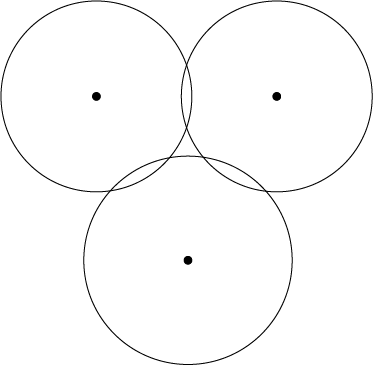
\includegraphics[width=0.4\textwidth]{vrdiag.png}
    \caption{The Vietoris-Rips complex generates a full triangle, while the Cech complex an empty one.}
    \label{fig:vrdiag}
\end{figure}

The Vietoris-Rips complex can be seen as a Cech complex in which the added complexes have all the faces included in Cech complex. It follows that the Cech complex is a subset of Vietoris-Rips complex. Of course in this case both complexes have the same parameter $\delta$. It's important to note that the Vietoris-Rips complex, similar to Cech complex, also has problems with high dimensional simplexes.

\subsection{Persistence}

Homology groups are one of the main concepts of algebraic topology. The topology is represented by the \emph{Betti numbers}, which represent the rank of the homology groups. Homology of degree 0 represents a connectedness of data (how many connected components are there), homology of degree 1 detects holes and tunnels, homology of degree 2 detects voids etc... In this assignment we limited our research to the first three important groups.

The connectedness of discrete points is represented with complexes. It depends on certain parameters like radius around the points, which tells us which points are interconnected. The connectedness therefore can't be defined universally.

This problem is solved by the concept of \emph{persistence}. The idea of persistence is, that by increasing the radius around the point, the complexes and homology groups also change. That however tells us which topology \emph{persists} through the changes.

In Image~\ref{homo} it can be observed that by increasing the radius, the graph becomes more connected. The lines in the diagram represent the ``life span'' of a topological feature. At some $\delta$ the number of crossed lines represents the Betti number for a specific degree. \cite{persist}

\begin{figure}[htb]
    \centering
    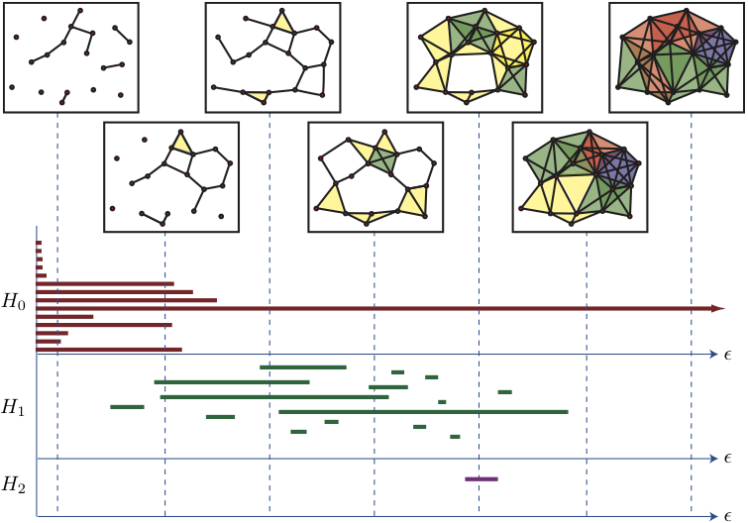
\includegraphics[width=0.8\textwidth]{homo.png}
    \caption{Persistence and the barcode diagram.}
    \label{homo}
\end{figure}

If we look at the second crossing, there are 6 connected components and two holes. In the assignment we filtered out all the entries that have the length of the line zero (is born and dies at the same delta).

Another way of using the persistence diagram is to plot the \emph{birth} and \emph{death} times of connected components (seen as lines in barcode diagram). Since each feature is represented by a $z = (birth, death)$ pair, we can plot this as points in a plane where the x-axis represents the birth of a feature and the y-axis it's death. Small features will have death times close to their birth times, which means they will be closer to the diagonal. The points near the diagonal can be looked at as \emph{topological noise} while those further away as \emph{topological signals}.


\section{Approach}

The data on which the rubustness of persistence diagrams was to be demonstrated was the set of points \emph{S}. Then the largest distance \emph{R} between any two points in the data set \emph{S} was found and was divided into parts of increasing size: $0 = r_0 < r_1 < r_2 < ... < r_n = R$. For every \emph{r} the Vietoris-Rips complexes $V_i = V_ri(S), i = 0,...,n$ were constructed. This represented a \emph{filtration} $V_0 \leq V_1 \leq ... \leq V_n$. For each \emph{$V_i$} the persistence diagrams of the filtration in dimensions 0, 1 and 2 were created. The whole process was repeated many times on shaken up data set, which was obtained by adding a small error term $\epsilon < R/100$ to the coordinates of each point in S.

We compared all the obtained persistence diagrams, which were also plotted in a single diagram, showing all the shaken up versions (and the original) of the same feature connected by a line. The diagrams were compared using bottleneck distance which compares a persistence diagram of a shaken up version of the dataset to the original version. The bottleneck distance measures how much we have to move the points in the shaken up persistence diagram to match the points from the original one.

% !!!!!!!!!!!!!!!! a kle je complex al kva ne lih point...  feature?

C++, Qt framework and the topological computation library Dyonisus were used to compute Vietoris-Rips complexes, while the diagrams were generated using Python.

\section{Problems}

We had some smaller problems, which were mostly solved by some compromises:

\begin{enumerate}
\item the dataset was too large, so we couldn't use the largest distance between two points, or the generation of Vietoris-Rips complex would take too long; we used an arbitrarily chosen value;

\item when computing the persistence diagram (une crte k skacejo na sliki)...

\item ...
\end{enumerate}

\section{Results}

% to bom se prevedu i guess
Z večanjem $\delta$ seveda narašča čas računanja. Alpha oblike delujejo hitreje kot vietoris-rips. Zelo zanimivo (in pravilno) je delovanje izračuna homologije, saj npr. pri krogli, v primeru, da ima ta 3 luknje, izračuna homologijo kot (1,2,0), torej 1 povezana komponenta in 2 tunela. V primeru, da imamo 4 luknje dobimo homologijo (1,3,0), torej 3 tuneli oz. če sploščimo dobljeno formacijo okol ene od lukenj dobimo 3 luknje (glej Sliko~\ref{lukne}).

%\begin{figure}[htb]
%    \centering
%    \includegraphics[width=1\textwidth]{lukne_primer.png}
%    \caption{Primer homologije pri krogli s 4 luknjami.}
%    \label{lukne}
%\end{figure}

$\delta$ parameter je tesno povezan s tipom podatkov. Pri gostejših oblakih bo zadostila manjša $\delta$. Podobno so lahko razdalje v setu točk zelo velike (čeprav je oblak zelo velik oz. gost), zato bo potrebna večja $\delta$. Iz slik v nadaljevanju je vidno delovanje programa. Program je prilo"zen v zip datoteki.



%\newpage % mogoce nav treba

\section{Work distribution}

% pac dodejte kej al sprementa al kokr se vama pac zdi fer... 

\subsection{Ožbolt}
Reading and formating of data, point shakeup, bottleneck distance, testing.

\subsection{Anej}
Vietoris-Rips, generation of diagrams.

\subsection{Jurij}
Project groundwork setup, ???, testing. % sry mal sm zaspan... pac dopis whatever, lohk da tut kej k sm pr ozboltu premakn k seb da bo pac vsak mel neki pa je mir...

\newpage

\bibliographystyle{plain}
\bibliography{report-bib}

\end{document}
